\documentclass[11pt,a4paper]{article}

% Packages
\usepackage[utf8]{inputenc}
\usepackage[spanish, es-tabla]{babel}
\usepackage{caption}
\usepackage{listings}
\usepackage{minted}
\usepackage{adjustbox}
\usepackage[colorlinks=true]{hyperref}
\usepackage[shortlabels]{enumitem}
\usepackage{boldline}
\usepackage{amssymb, amsmath}
\usepackage{amsthm}
\usepackage{subcaption}
\usepackage[noend]{algpseudocode}
\usepackage[margin=1.2in]{geometry}
\usepackage{xcolor}
\usepackage{soul}
\usepackage{upgreek}

%\usemintedstyle{bw}

\decimalpoint

\hypersetup{
  allcolors=magenta
}

% Meta
\title{Gestión de Datos\\ \Large{Exploración gráfica de datos} }
\author{Luis Antonio Ortega Andrés\\Antonio Coín Castro}
\date{\today}

% Custom
\providecommand{\abs}[1]{\lvert#1\rvert}
\setlength\parindent{0pt}
% Redefinir letra griega épsilon.
\let\epsilon\upvarepsilon
% Fracciones grandes
\newcommand\ddfrac[2]{\frac{\displaystyle #1}{\displaystyle #2}}
% Primera derivada parcial: \pder[f]{x}
\newcommand{\pder}[2][]{\frac{\partial#1}{\partial#2}}

\newcommand{\fx}{\frac{1}{\sqrt{2\pi}\sigma} e^{\frac{-(x-\mu)^2}{2\sigma^2}}}
\newcommand{\R}{\mathbb{R}}

\begin{document}
\maketitle

\section{Problema a resolver}
En este ejercicio pretendemos explorar visualmente un dataset para obtener información sobre los datos que representa. Concretamente, usaremos el lenguaje R para explorar un dataset\footnote{\href{http://cardsorting.net/tutorials/25.csv}{http://cardsorting.net/tutorials/25.csv}} resultado de un Card Sorting sobre alimentos. Nos interesa la siguiente información:

\begin{enumerate}
  \item Tipología y rango de los datos numéricos.
  \item Tarjetas más relacionadas entre sí.
\end{enumerate}

\section{Lectura y limpieza de datos}

En primer lugar, leemos los datos desde el recurso remoto empleando la función \textit{built-in} de R \verb@read.csv@. La estructura de datos principal que usaremos será el dataframe, por lo que también haremos uso de las funciones de R para manipularlos. Como solo nos interesa estudiar los datos numéricos, prescindimos de las columnas \textit{Uniqid, Startdate, Starttime, Endtime, QID} y \textit{Comment}. Para ello usamos la orden \verb@subset@ que nos permite quedarnos solo con columnas específicas del dataframe.

\section{Estudio de los datos numéricos}

Nos preguntamos qué tipos de datos numéricos alberga el dataset, así como el rango de los mismos. Para visualizar esta información, prescindimos momentáneamente de la columna \verb@Category@ (que sabemos que es la única restante que no es numérica) y realizamos un histograma de los datos. El resultado obtenido podemos verlo en la Figura \ref{fig:1}. Como se puede apreciar, el conjunto está formado únicamente por valores binarios (0 ó 1), y además la proporción de 0s es mucho mayor (casi 10 veces mayor). Podemos concluir entonces que el dataset está configurado de forma que las observaciones están ``desagrupadas''; es decir, por cada fila tenemos una observación de un usuario en una categoría concreta, habiendo un $1$ en aquellas tarjetas que ha estimado que pertenecen a dicha categoría.

\begin{figure}[h!]
  \centering
  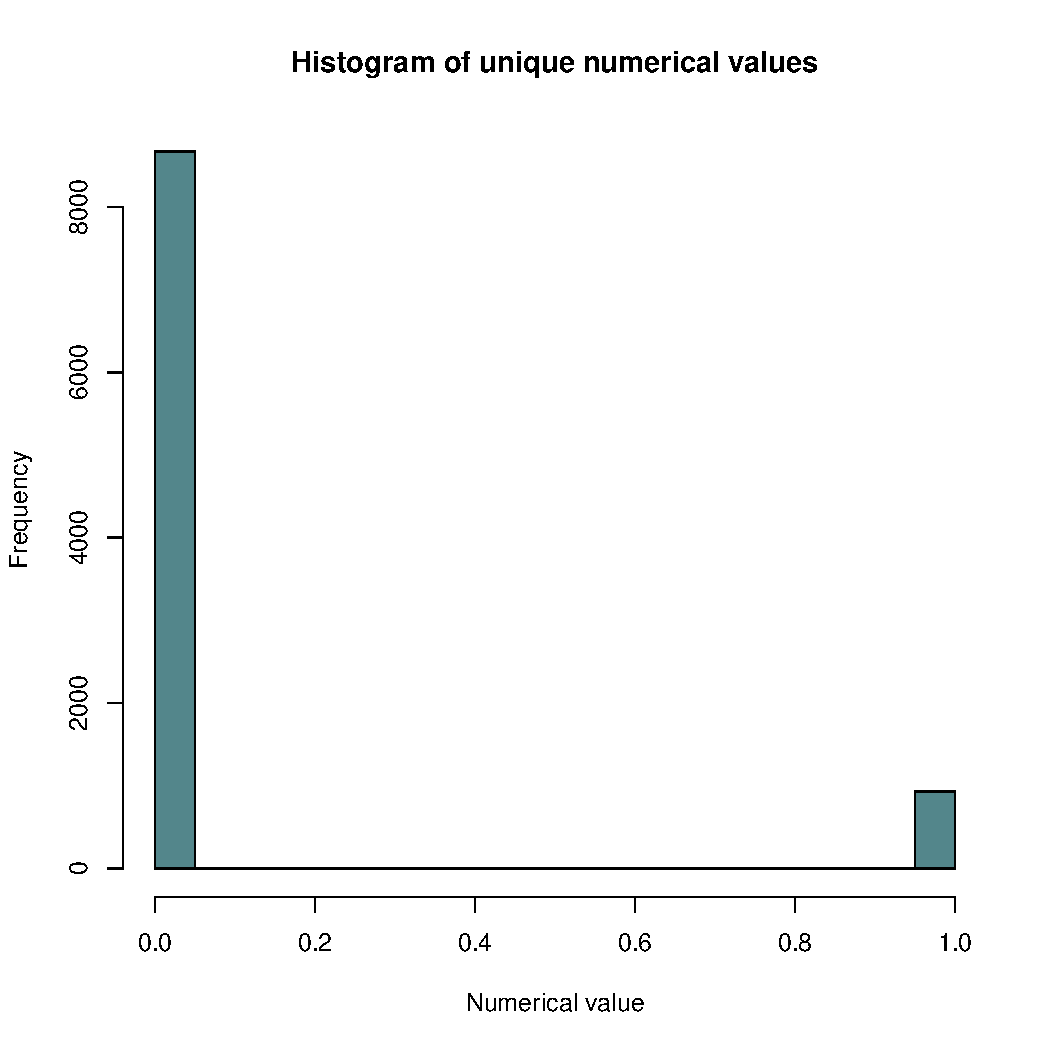
\includegraphics[page=1, width=.7\textwidth]{Rplots.pdf}
  \caption{Histograma de los datos numéricos.}
  \label{fig:1}
\end{figure}

\section{Similitud entre tarjetas}

Nos preocupamos ahora de estudiar cómo se relacionan las diferentes tarjetas a la luz de los datos de los que disponemos. Como primer enfoque, calculamos una \textbf{matriz de distancias} entre las mismas, de forma que podamos cuantificar cómo de cerca están las unas de las otras. La métrica que elegimos para hacer esto es la métrica euclídea, de forma que cada componente represente una categoría. Así, la contribución de las categorías donde las tarjetas coincidan será nula, mientras que aquellas para las que no coincidan contribuirán con un factor de $1$ en la suma correspondiente. Para calcular esta matriz usamos la función \verb@dist@ de R.\\

Por otro lado, para visualizar la matriz de distancias empleamos un enfoque doble: hacemos un mapa de calor y un dendrograma. Estos dos gráficos suelen ir de la mano, y de hecho el comando \verb@heatmap.2@ de la librería \verb@gplots@ los pinta a la vez por defecto. El resultado para nuestra matriz de distancias entre tarjetas se observa en la Figura \ref{fig:2}.\\

\begin{figure}[h!]
  \centering
  \includegraphics[page=2, width=0.7\textwidth]{Rplots.pdf}
  \caption{Mapa de calor y dendrograma asociado a las distancias.}
  \label{fig:2}
\end{figure}

Lo que nos interesa es medir la similitud de las tarjetas, entendiendo que se parecerán cuando coincidan un número elevado de categorías en las que se ordenan. En el mapa de calor se puede observar cómo hay varios grupos o \textit{clústers} de tarjetas a poca distancia, representadas por el color rojo/naranja oscuro. Esta misma información se puede obtener del dendrograma, viendo como algunas categorías no se dividen hasta casi el final del eje. Ambas representaciones se complementan bastante bien, haciendo que de un vistazo podamos obtener la información que buscamos.\\

Finalmente, podemos estudiar las relaciones entre las tarjetas mediante un grafo, donde los nodos serán las tarjetas y todos estarán relacionados con todos. El peso de las conexiones será la similitud entre las tarjetas que representan, haciendo que visualmente las líneas sean más gruesas cuanto más similares sean. Para visualizar esto utilizamos la función \verb@qgraph@ de la librería homónima, teniendo en cuenta que debemos pasar una matriz de similitud y no una matriz de distancia. Como métrica de similitud escogemos, por ejemplo, la matriz de los inversos de las distancias, de forma que sean todas positivas y aumenten conforme menor sea la distancia. El resultado se puede ver en la Figura \ref{fig:3}.

\begin{figure}[h!]
  \centering
  \includegraphics[page=3, width=0.7\textwidth]{Rplots.pdf}
  \caption{Representación mediante un grafo ponderado de la similitud entre tarjetas.}
  \label{fig:3}
\end{figure}

\section{Tarjetas más relacionadas y significado semántico}

Utilizando la representación en grafo de las similitudes, es bastante sencillo localizar las tarjetas más similares. En concreto, tenemos un grupo de tarjetas muy parecidas: \textbf{Banana, Apple, Watermelon, Pineapple} y \textbf{Orange}. También tenemos otros grupos de tarjetas parecidas, como \textbf{Pie} y \textbf{Cake}; \textbf{Salmon} y \textbf{Lobster}; \textbf{Pancake} y \textbf{Waffle}, y también \textbf{Brocoli}, \textbf{Carrots} y \textbf{Lettuce} (y en este último también en menor medida, \textbf{Onion}).\\

Podemos comprobar que efectivamente todos los grupos que hemos mencionado arriba tienen la distancia minimal entre ellos (de entre todas las tarjetas), utilizando las órdenes \verb@min@ y \verb@which@ de R. Esta distancia es $\sqrt{2}$, es decir, que las tarjetas más parecidas coinciden en todas las categorías excepto en 2. Además, podemos ver que los grupos obtenidos tienen sentido desde un punto de vista semántico: el primero representa frutas, el segundo postres y cosas dulces; el tercero pescado, y el cuarto verduras y hortalizas.\\

Como último paso de este análisis, podemos echar un vistazo a las categorías en las que han sido clasificadas algunas de las tarjetas más parecidas. Por ejemplo, los histogramas de categorización para \textbf{Apple} y \textbf{Banana} pueden verse en la Figura \ref{fig:4}, mientras que los de \textbf{Pie} y \textbf{Cake} está representados en la Figura \ref{fig:5}. Como vemos, las categorías más frecuentes para los dos primeros son aquellas que de alguna forma describen frutas, y para los dos últimos son categorías que representan dulces, postres o comida rápida\footnote{Notamos que lo que estamos representando en el histograma es la frecuencia con la que se elige cada categoría; no es una comparación de cuándo coincide y cuando no la categorización de las dos tarjetas para un usuario en concreto.}. Sin disponer de información adicional no podemos interpretar las categorías que se han codificado como un número, pero aun así dentro de las tarjetas similares hay algunas categorías en esta situación que han coincidido para 2 o más usuarios.

\begin{figure}[h!]
  \centering
  \includegraphics[page=4, width=0.7\textwidth]{Rplots.pdf}
  \caption{Histogramas de categorías en las que han sido colocados Apple y Banana.}
  \label{fig:4}
\end{figure}

\begin{figure}[h!]
  \centering
  \includegraphics[page=5, width=0.7\textwidth]{Rplots.pdf}
  \caption{Histogramas de categorías en las que han sido colocados Pie y Cake.}
  \label{fig:5}
\end{figure}

\end{document}
